This chapter focuses on the design and implementation aspects of developing vision-based control solutions for UAVs within the PX4 ecosystem. It begins by discussing simulation as a safe and cost-effective environment for exploring and refining algorithms without the risks associated with real-world flights. The implementation of simulation in PX4 is explored, covering components such as the simulated flight stack and the simulation engine. The specific simulation and development environment for this project, including system configurations and the use of Unreal Engine and AirSim as the simulation engine, is also examined.

The chapter then moves on to describe the system architecture of the interaction between the flight controller and the DroneVisionControl application running on a companion computer. It discusses two possible hardware configurations: one where the companion computer remains on the ground when the drone flies (offboard configuration) and another where it is placed onboard the vehicle during flight. The key components of the system, including the flight controller, companion computer, and camera, are outlined, along with the methods to exchange information between them. Furthermore, the software architecture of the DroneVisionControl application is described, highlighting the modules that make up the application.

To conclude, two control solutions are presented which demonstrate the capabilities of the PX4 ecosystem. The first one (Section \ref{sec:hands} - Hand-gesture solution) is designed for the offboard configuration as a proof-of-concept solution where the vehicle is controlled from a ground station by hand gestures. The second (Section \ref{sec:follow} - Follow solution) demonstrates the applications of the onboard configuration with a person-following solution that makes the drone fly to maintain a moving person centred in its field of view.

\section{Simulation and development environment}
\label{sec:devenv}
Simulation plays a crucial role in developing vision-based control solutions for UAVs. It offers a safe and cost-effective environment to explore and refine algorithms, test new capabilities, and evaluate system performance without the risks associated with real-world flights. 
In this context, simulation refers to creating a computer-generated virtual environment that mimics a UAV's real-world conditions and interactions. In this simulation, various aspects of the UAV system, including the flight dynamics, sensor inputs, and environmental factors, are replicated and simulated in a software-based environment.

This section explores how simulation is implemented in the PX4 platform and the development environment built around it for this project to develop the hand-gesture and follow control solutions mentioned before.
The three key simulation components are examined individually: the simulated flight stack, the simulation engine or simulator, and the companion computer for offboard control. 
The two available simulation modes, \acrfull{sitl} and \acrfull{hitl}, are introduced for the flight stack. In contrast, the simulation engine encompasses modelling physical world components and the physics and rendering engines. 
The communication between the simulator, flight controller firmware, and companion computer is also described. 
Lastly, the development environment is discussed, covering network configurations and using Unreal Engine and AirSim as the simulation engine for this project.

\subsection{SITL and HITL simulation}

The PX4 platform is a flexible and powerful open-source flight control software stack widely used for developing for UAVs. The platform’s flight stack is the core software responsible for controlling the UAV's behaviour and executing flight commands. It offers comprehensive support for simulation, providing developers with a robust environment to test and refine their control solutions.

There are two main simulation modes for the flight stack: \acrfull{sitl} and \acrfull{hitl}. SITL simulation enables the flight stack to run on a non-dedicated computer, simulating the flight controller’s operating system and allowing for rapid development and testing. On the other hand, HITL simulation executes the simulation firmware on an actual flight controller board, providing a more realistic testing environment. In this mode, the flight stack runs in its native environment while the sensor data and other external inputs are simulated.

Both simulation modes in the PX4 platform offer distinct advantages and are suited for different stages of development. SITL simulation allows developers to iterate quickly, reducing development time and providing immediate visual feedback on the computer screen. This mode is particularly beneficial during algorithm exploration and refinement. HITL simulation, on the other hand, offers increased realism by testing on an actual flight controller board. It allows developers to evaluate their vision-based control solutions in a more accurate representation of the real-world environment. This mode is especially valuable when fine-tuning algorithms and assessing system performance.

In the simulation context, two inextricable components exist: the simulated flight stack (running on SITL or HITL mode) and the simulation engine or simulator. The flight stack interacts with the simulator through a feedback loop, enabling a seamless exchange of information between the two components, as shown in Figure \ref{fig:simulator-loop}.
The feedback loop begins with the simulator generating sensor inputs, such as acceleration measurements or GPS data, based on its internal representation of the simulated world. These sensor inputs are then transmitted to the flight stack.
Upon receiving the sensor inputs, the flight stack processes this information and generates response actuator controls, including motor commands or control signals for various UAV components, which are then sent back to the simulator. Finally, the simulator utilises these actuator controls to update the virtual vehicle's position, velocity, and attitude within the simulated world, thereby simulating the UAV's response to the flight stack's commands. 

This interaction between the flight stack and the simulator within the feedback loop allows for a dynamic and synchronised simulation experience, mimicking the behaviour of a real-world UAV by providing realistic sensor inputs and simulating the corresponding actuator responses.
All communication between the flight stack and the simulator is implemented using the MAVLink messaging protocol and the UDP transport protocol. MAVLink messages serve as a standardised format for transmission, allowing the seamless exchange of information between the two components.

\begin{figure}
  \centering
  
\includegraphics[width=\textwidth,keepaspectratio]{img/px4-simulator-loop.png}
  \caption{Feedback loop during the PX4 simulation.}
  \source{Adapted from \citetitle{px4-guide} \cite{px4-guide}.}
  \label{fig:simulator-loop}
\end{figure}

\subsection{Simulator}


\begin{figure}
  \centering
  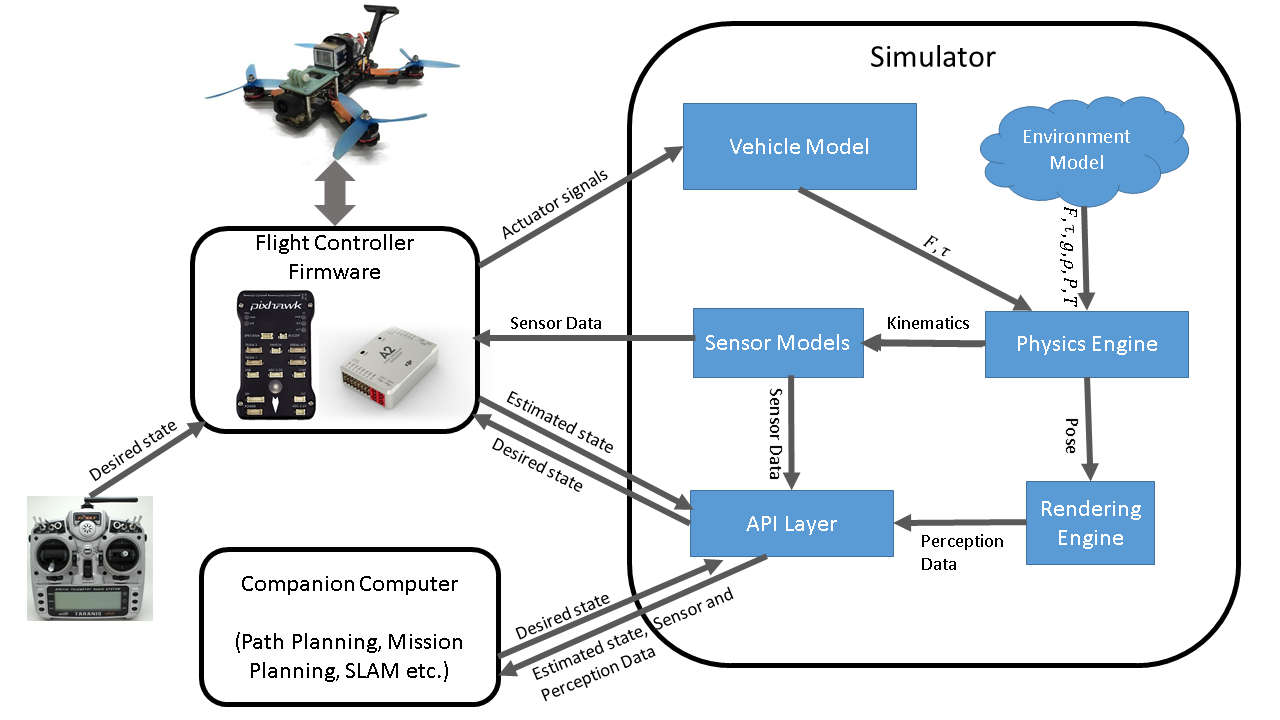
\includegraphics[width=\textwidth,keepaspectratio]{img/airsim-overview.png}
  \caption{High-level overview of how different components of a simulator interact with the flight stack.}
  \source{Adapted from \citetitle{airsim-paper} \cite{airsim-paper}.}
  \label{fig:airsim-overview}
\end{figure}

The simulator plays a crucial role in development by providing visual feedback on the vehicle’s reactions to the control software.
Inside the simulator, a group of components that model real-world elements work together to make up the complete engine.
Figure \ref{fig:airsim-overview} expands upon the diagram in Figure \ref{fig:simulator-loop} to show the high-level overview of how each of these components interacts with each other and with the flight controller firmware (flight stack).

The environment model represents the virtual world where the simulation occurs, providing the simulated surroundings and obstacles for the UAV. It can include terrain and weather conditions that affect flight dynamics, like wind or variable temperatures, which are sent to the physics engine. 
The vehicle model represents the UAV's physical characteristics, such as its mass, size, aerodynamics, and propulsion system, which are simulated to generate forces and moments based on actuator signals.
The sensor model simulates the behaviour and outputs of cameras, lidars, and \acrshort{imu}s, providing realistic sensor data to the flight stack.
The physics engine governs the laws of physics within the simulation, calculating forces, torques, collisions, and other physical interactions to ensure that the vehicle and its environment interact realistically.
The rendering engine is responsible for rendering the visual aspects of the simulation, allowing for realistic graphics and visualisation.
The final component of the simulator is the \acrshort{api} layer. It serves as a communication interface between the simulator and the flight stack, facilitating the exchange of data and control commands through the MAVLink protocol. This API can also connect the simulator to an external companion computer to use the sensor and state data provided. 

In this context, the companion computer is an additional computational device that works together with the flight controller firmware and the simulator. It aims to offload specific tasks and computations from the flight controller, enabling more complex algorithms, higher-level control, and real-time data processing. The companion computer allows implementing vision-based control solutions, as it can handle intensive image processing and machine learning. It facilitates the integration of advanced perception, planning, and decision-making capabilities, enhancing the UAV's autonomy and enabling more sophisticated behaviours in simulated environments.
The communication between the companion computer and the simulation system can be established by the simulator’s own API layer, as shown in Figure \ref{fig:airsim-overview}, or through any dedicated API that can interact with the flight stack through MAVLink messages.
An example of the latter case would be the MAVSDK API mentioned in Section \ref{subsec:mavlink}.
MAVSDK is used in this project to isolate the communication between the flight stack and the companion computer from the simulator.
This separation allows for a more seamless transition into flight tests, where the real world replaces the simulator component.

There are many options for simulators supported by PX4.
The simpler of these is jMAVSim, which can be installed along with the PX4 SITL simulation on a Linux system. It provides a lightweight simulation environment for PX4, allowing for basic testing and evaluation of flight control algorithms. While it may lack some advanced features like supporting complex simulated worlds, jMAVSim is a convenient option for checking that the simulated flight stack has been configured correctly during initial development iterations.
A second option for running on Linux is Gazebo. Gazebo is a powerful simulator widely used in robotics and compatible with PX4. It offers more advanced capabilities, such as obstacle avoidance and support for the Robot Operating System (ROS). It provides a realistic physics engine for simulating UAV dynamics and environments and enables the integration of complex sensor models, making it suitable for testing perception and navigation algorithms. However, it is more limited in graphics, which becomes critical when testing control solutions driven by computer vision.

The last option considered to fulfil the requirements of the project is AirSim. This simulator is built as a plugin for the popular Unreal Engine, designed for game development. Unlike jMAVSim and Gazebo, AirSim runs on Windows and leverages the capabilities of a game engine. It provides visually and physically realistic simulations, offering advanced graphics and rendering capabilities. AirSim is particularly advantageous for testing computer vision features as it offers easy access to thousands of visual packages through its asset library. Its integration with Unreal Engine enables the creation of complex and immersive simulated environments. These features make it especially suited for developing vision-based control solutions, making it the best choice for this project.


\subsection{Development environment}

This section discussed the configuration adopted in this project to establish connections between the developed control software, the selected AirSim simulator, and the flight stack. It encompasses both SITL and HITL simulation modes, which allow testing the implementation of the DroneVisionControl application within a controlled environment. While the application is designed to leverage the dedicated processing power of a companion computer in real-world scenarios, during simulation, it will primarily operate on the same computer hosting the simulation engine to minimise physical connections between multiple machines.

\subsubsection{SITL configuration}

\todo[inline]{Fix this graph}
\begin{figure}
  \centering
  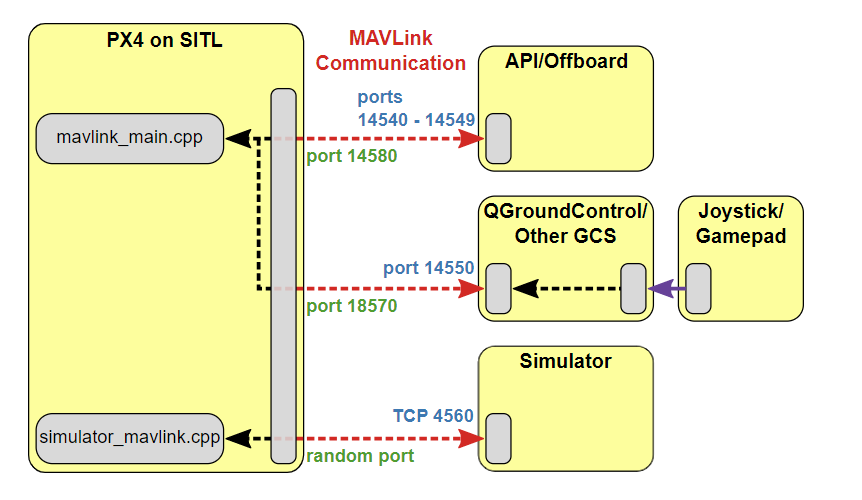
\includegraphics[width=\textwidth,keepaspectratio]{img/px4-ports.png}
  \caption{Network diagram between the components interconnecting during software-in-the-loop simulation.}
  \source{Adapted from \citetitle{px4-guide} \cite{px4-guide}.}
  \label{fig:px4-ports}
\end{figure}

The PX4 platform has an established network configuration for SITL simulation, shown in Figure \ref{fig:px4-ports}. The figure’s left side shows the two programs that manage MAVLink servers for communicating with components outside the flight stack. The first is the main MAVLink manager, inherent to the PX4 system. It expects connections from offboard control sources, such as a companion computer using an offboard API (MAVSDK) or a ground control station like QGroundControl (\ref{subsec:qgc}). These connections are established using the \acrshort{udp} protocol on the port range 14540-14550. By default, port 14550 is reserved for a ground station but can be used by any other offboard application if \acrshort{qgc} is not required.
The second server runs exclusively during simulations and connects to the simulator program instead through a \acrshort{tcp} connection, as it requires higher reliability than the offboard connections.

In this project, the simulator will run on a Windows system, as that is the native environment of the AirSim simulator. The SITL simulation, however, runs best on Linux. To execute both software components simultaneously on a single machine, the \acrfull{wsl} \cite{wsl-learn} will be utilised. WSL allows for the execution of a Linux distribution, such as Ubuntu, directly within the Windows operating system, providing a convenient environment for running PX4 SITL alongside AirSim without the need for dual-booting or virtual machines. This configuration ensures that the connections are limited to the machine’s internal network, as WSL handles the task of establishing network connectivity between the Windows and Linux environments. It achieves this by setting up a virtual Ethernet bridge and ensuring network traffic is routed appropriately.
The complete steps needed to configure the PX4 WSL system are detailed in Appendix \ref{app:install-dev-env}.


\begin{figure}
  \centering
  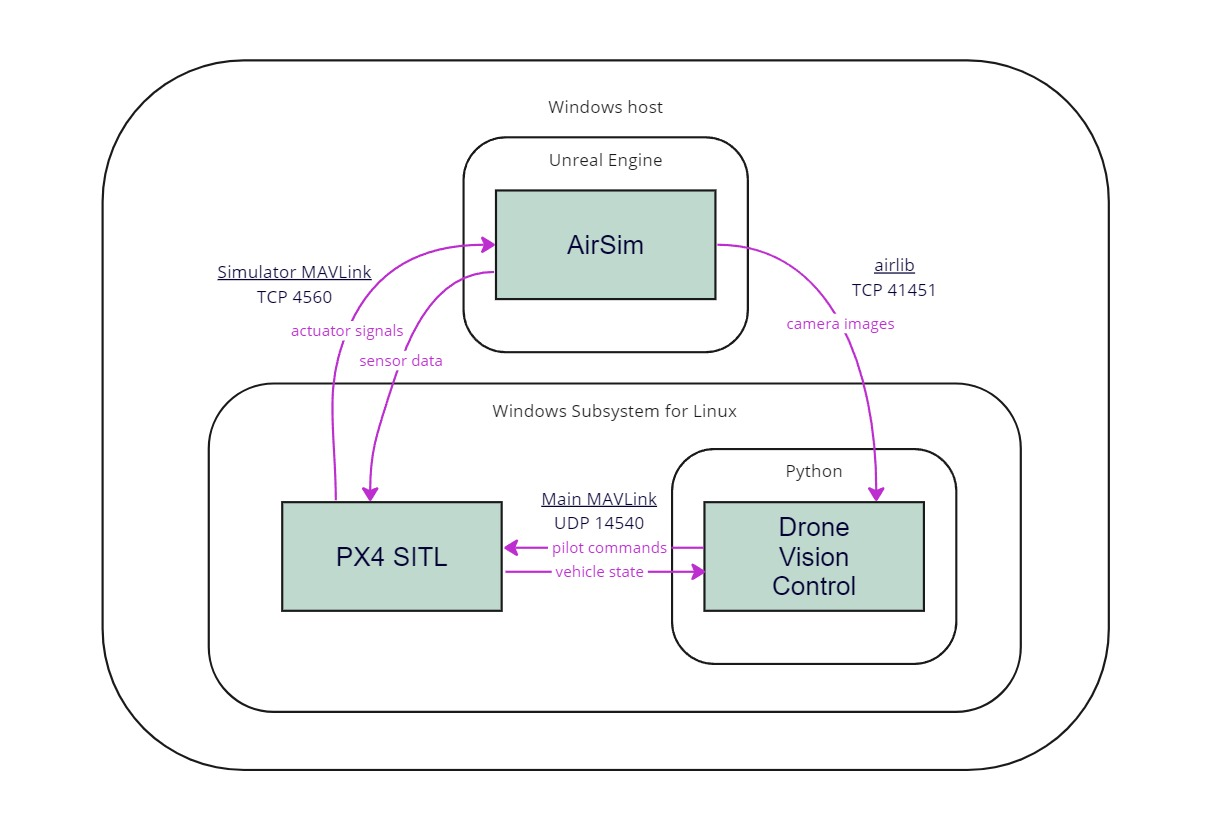
\includegraphics[width=0.8\textwidth,keepaspectratio]{img/sitl-connections.jpg}
  \caption{Connection diagram of how the three systems interact with each other during SITL simulation.}
  \label{fig:sitl-connections}
\end{figure}

The complete set of connections necessary between the three individual components at the transport layer level during SITL simulation is shown in Figure \ref{fig:sitl-connections}.
The AirSim simulator runs as part of the Unreal Engine application directly on the host Windows system. It connects to the other two components running inside the virtualised Linux subsystem through the established bridge. AirSim and the PX4 flight stack exchange information through the TCP connection to the secondary MAVLink server, as shown in Figure \ref{fig:px4-ports}.

The communication between AirSim and the DroneVisionControl application is facilitated through the API layer depicted in Figure \ref{fig:airsim-overview}, which can connect the simulator with a companion computer or other system running additional code. This connection is established using the \texttt{airlib} library developed for Python by the creators of AirSim, which allows easy access to the AirSim API. In this project, the connection between AirSim and the application through \texttt{airlib} transmits only perception data, specifically camera images of the simulated world. 
For the transmission of other data, such as the current vehicle state from the simulator to the application and the desired state from the application to the simulator, the PX4 flight stack will be used as an intermediary. This way, the DroneVisionControl application does not need to be concerned with whether the flight mechanics are being simulated or determined by sensors in the real world. The link between the developed application and the flight stack is established through the main MAVLink instance, as shown in Figure \ref{fig:px4-ports} (\texttt{mavlink\_main.cpp}).

Given that the application is developed in Python, a versatile programming language compatible with multiple platforms, it can be run either on the central Windows system or within the virtualised Linux subsystem. However, running the application on Linux is more advantageous to avoid the need for the MAVLink server to broadcast to the Windows system.



\subsubsection{HITL configuration}

\begin{figure}
  \centering
  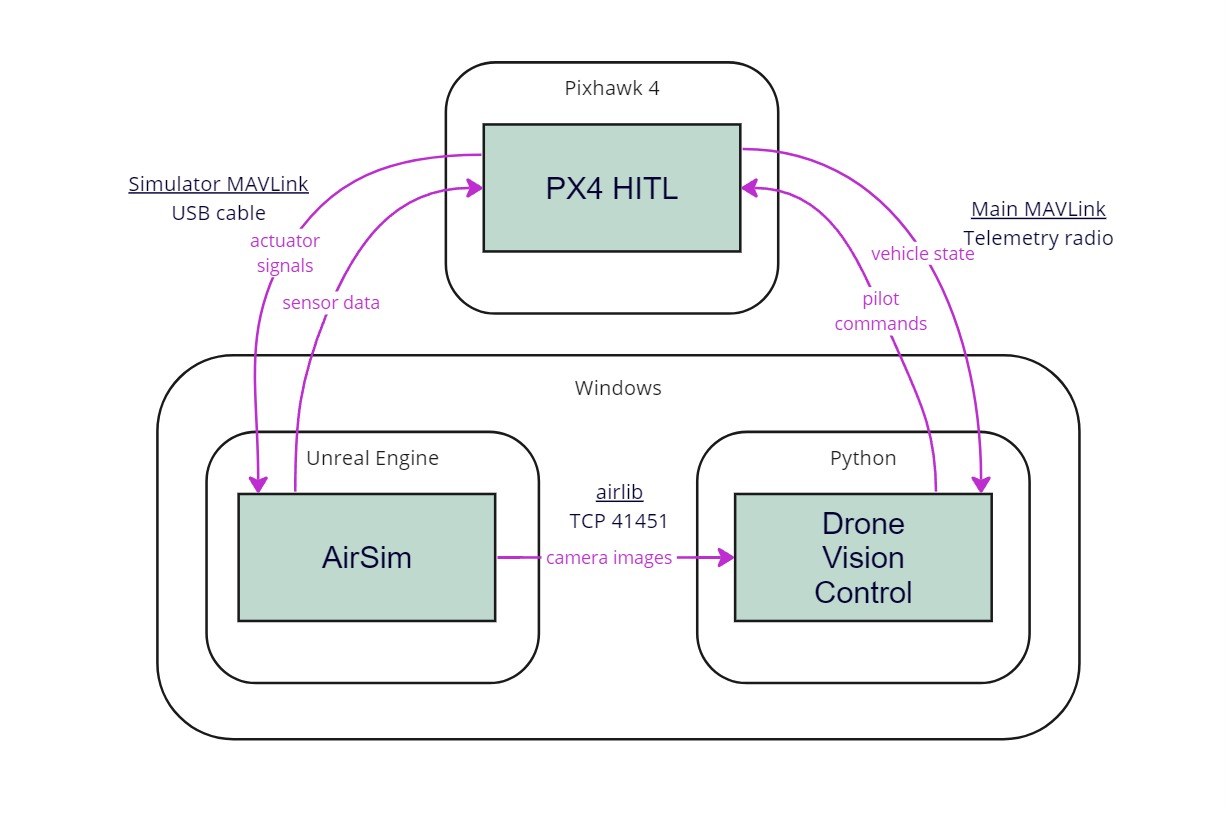
\includegraphics[width=0.8\textwidth,keepaspectratio]{img/hitl-connections.jpg}
  \caption{Connection diagram of how the three systems interact with each other during HITL simulation.}\label{fig:hitl-connections}
\end{figure}

Transitioning from SITL to HITL simulation involves shifting from the WSL environment to a physical flight board, specifically a Pixhawk flight controller, to run the flight stack firmware. In HITL simulation, the flight board's motors and actuators are blocked, but the internal software functions fully. The Python execution will also be moved from the Linux subsystem to the Windows host. This transition simplifies the testing process by eliminating the need for additional configurations to establish communication between the flight controller and the internal WSL network, which is isolated from external machines by default.

As the flight stack now runs on separate hardware, it becomes necessary to establish a physical connection between the testing computer and the flight controller for each desired MAVLink channel. This connection can be set up using the debug micro-USB port or any available telemetry port on the flight controller. To use the telemetry ports to connect to a computer, it is necessary to use either a serial-to-USB converter or a pair of telemetry radios. The simulator and the Python application can communicate independently with the flight controller by using several of these options simultaneously to establish separate communication channels.

Figure \ref{fig:hitl-connections} illustrates the chosen connections for executing tests in HITL mode. The Windows machine hosts both AirSim in Unreal Engine and the Python interpreter running the developed application, which keep their communication through the \texttt{airlib} library. In this case, there is no need for the virtual bridge network, and the TCP connection is established through the \texttt{loopback} network. The PX4 flight controller is connected to the simulator via a USB to micro-USB cable, configured with a baud rate of 115200. It is also connected to the Python program through a telemetry radio operating at a baud rate of 57600. Both connections on the Windows computer side are attached to USB ports. These ports are accessible via their respective COM addresses, which must be specified in the configuration for AirSim and MAVSDK.


\subsubsection{AirSim environment}

Microsoft develops the AirSim simulator as a plugin in the computer graphics and game development program Unreal Engine.
It implements sensor, vehicle and environment models appropriate for flight simulation while taking advantage of the physics and rendering engines integrated into Unreal.
In the engine, a "project" comprises one or more environments where components like 3D models, cameras, and lighting can be added.
The source code for the AirSim project includes a basic Unreal environment with all the minimum components already configured that can be used to test the implementation or as a starting point for more complex environments. It contains several 3D shapes like blocks and spheres and a simple quadcopter to act as the simulated vehicle.
Creating custom Unreal environments and running AirSim inside them is also possible by manually adding the built plugin and a vehicle to an existing project.

The environment used in this project for testing the DroneVisionControl application is derived from the base AirSim environment and can be found on the project’s repository\footnote{\url{https://github.com/l-gonz/tfg-giaa-dronecontrol/tree/main/data}}. It contains a test quadcopter vehicle and some 3D shapes used as obstacles. The vehicle model also includes a virtual camera that allows retrieving images from the vehicle’s point of view in the simulated world.
The main addition to the default environment for this project is the 3D model of a human figure, to be used for testing the person detection and tracking mechanisms in the computer vision solution. The source of this model is a free asset library of human models made by Renderpeople \cite{render-people} obtained from the Unreal Marketplace. Some minor modifications have also been made to the background shapes and colours to provide better contrast for the camera. Figure \ref{fig:unreal-env} shows an image of the testing environment as seen from the Unreal viewport in Edit mode.


\begin{figure}
  \centering
  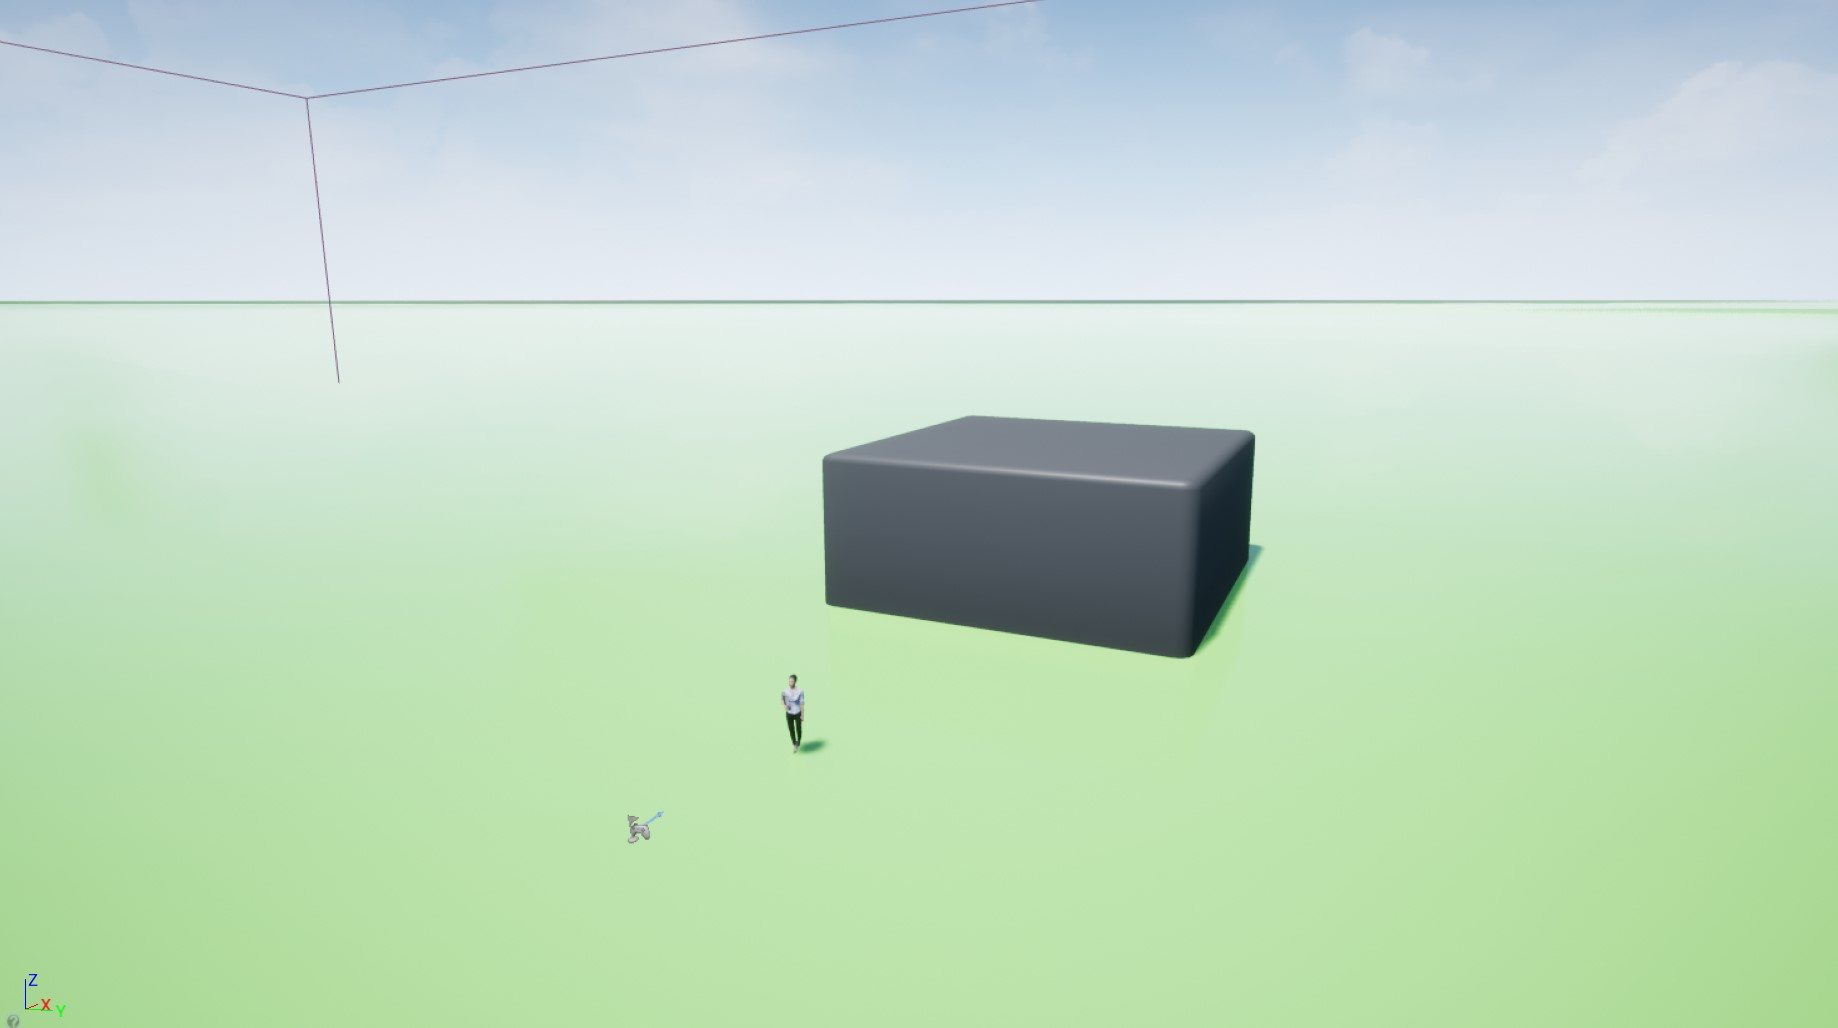
\includegraphics[width=\textwidth,keepaspectratio]{img/unreal-env.jpg}
  \caption{Screenshot from the Unreal Engine environment used for testing the computer vision solutions.}
  \label{fig:unreal-env}
\end{figure}


AirSim is compatible with both SITL and HITL simulation modes and several other flight stacks apart from PX4, including AirSim’s own internal SimpleFlight flight stack, which is used by default. 
The plugin must therefore be configured for this project to work with the desired simulation setup (PX4 + WSL + Airsim).
This process is explained in the AirSim documentation \cite{build-airsim} by its developers and in Appendix \ref{app:install-dev-env} for more project-specific details.
Appendix \ref{app:airsim-config} contains the complete settings file used in this project for configuring PX4 with either simulation mode in AirSim, including the parameters that must be individualised for each system.


To start the simulation in AirSim, the following steps must be followed:
\begin{enumerate}
 \item Attach physical flight controller in HITL mode to simulation computer (HITL only).
 \item Start play mode in Unreal.
 \item Build and start simulated flight stack in WSL (SITL only).
 \item Start companion applications, if any (e.g. DroneVisionControl, QGroundControl).
\end{enumerate}

To build and start the PX4 SITL flight stack for AirSim, a small script can be found in the project source code\footnote{\url{https://github.com/l-gonz/tfg-giaa-dronecontrol/blob/main/simulator.sh}} that will automatically attach to a running AirSim instance if it is executed with the \texttt{-{}-airsim} option.
To be able to use the physical flight board for HITL simulation, this mode needs to be enabled from the QGroundControl safety configuration.
Once the simulation has started, there is no noticeable change between the simulated flight controller in WSL (SITL mode) and the one running in the physical board (HITL mode).
